\section{Experiment}
\begin{figure}[H]
    \centering
    \begin{subfigure}{\textwidth}
        \centering
        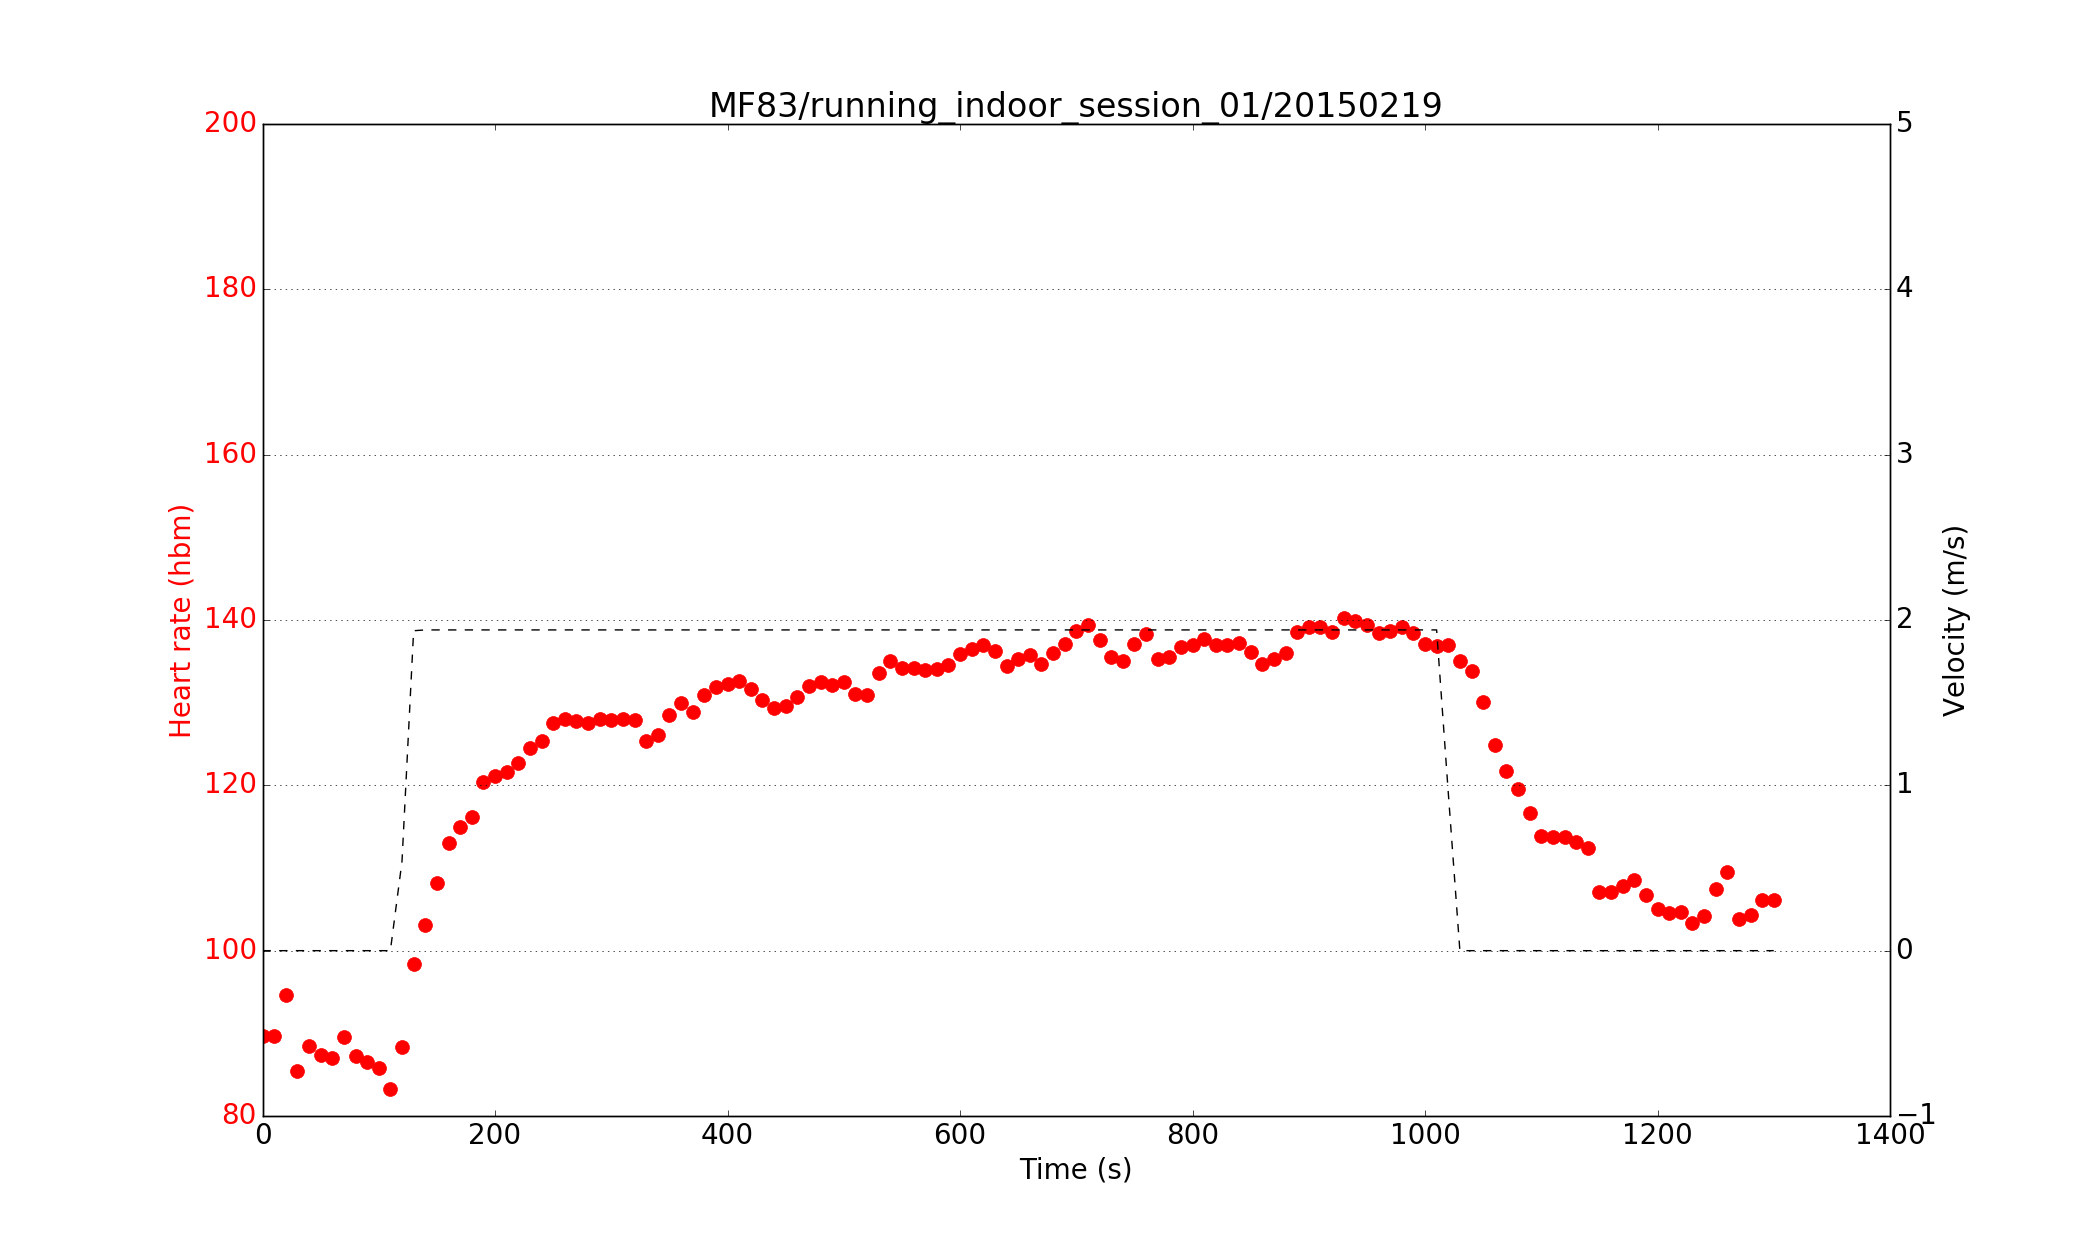
\includegraphics[height=6cm]{../images/plot_hbm_velocity-session1.png}
    \end{subfigure}%
    
    \begin{subfigure}{\textwidth}
        \centering
        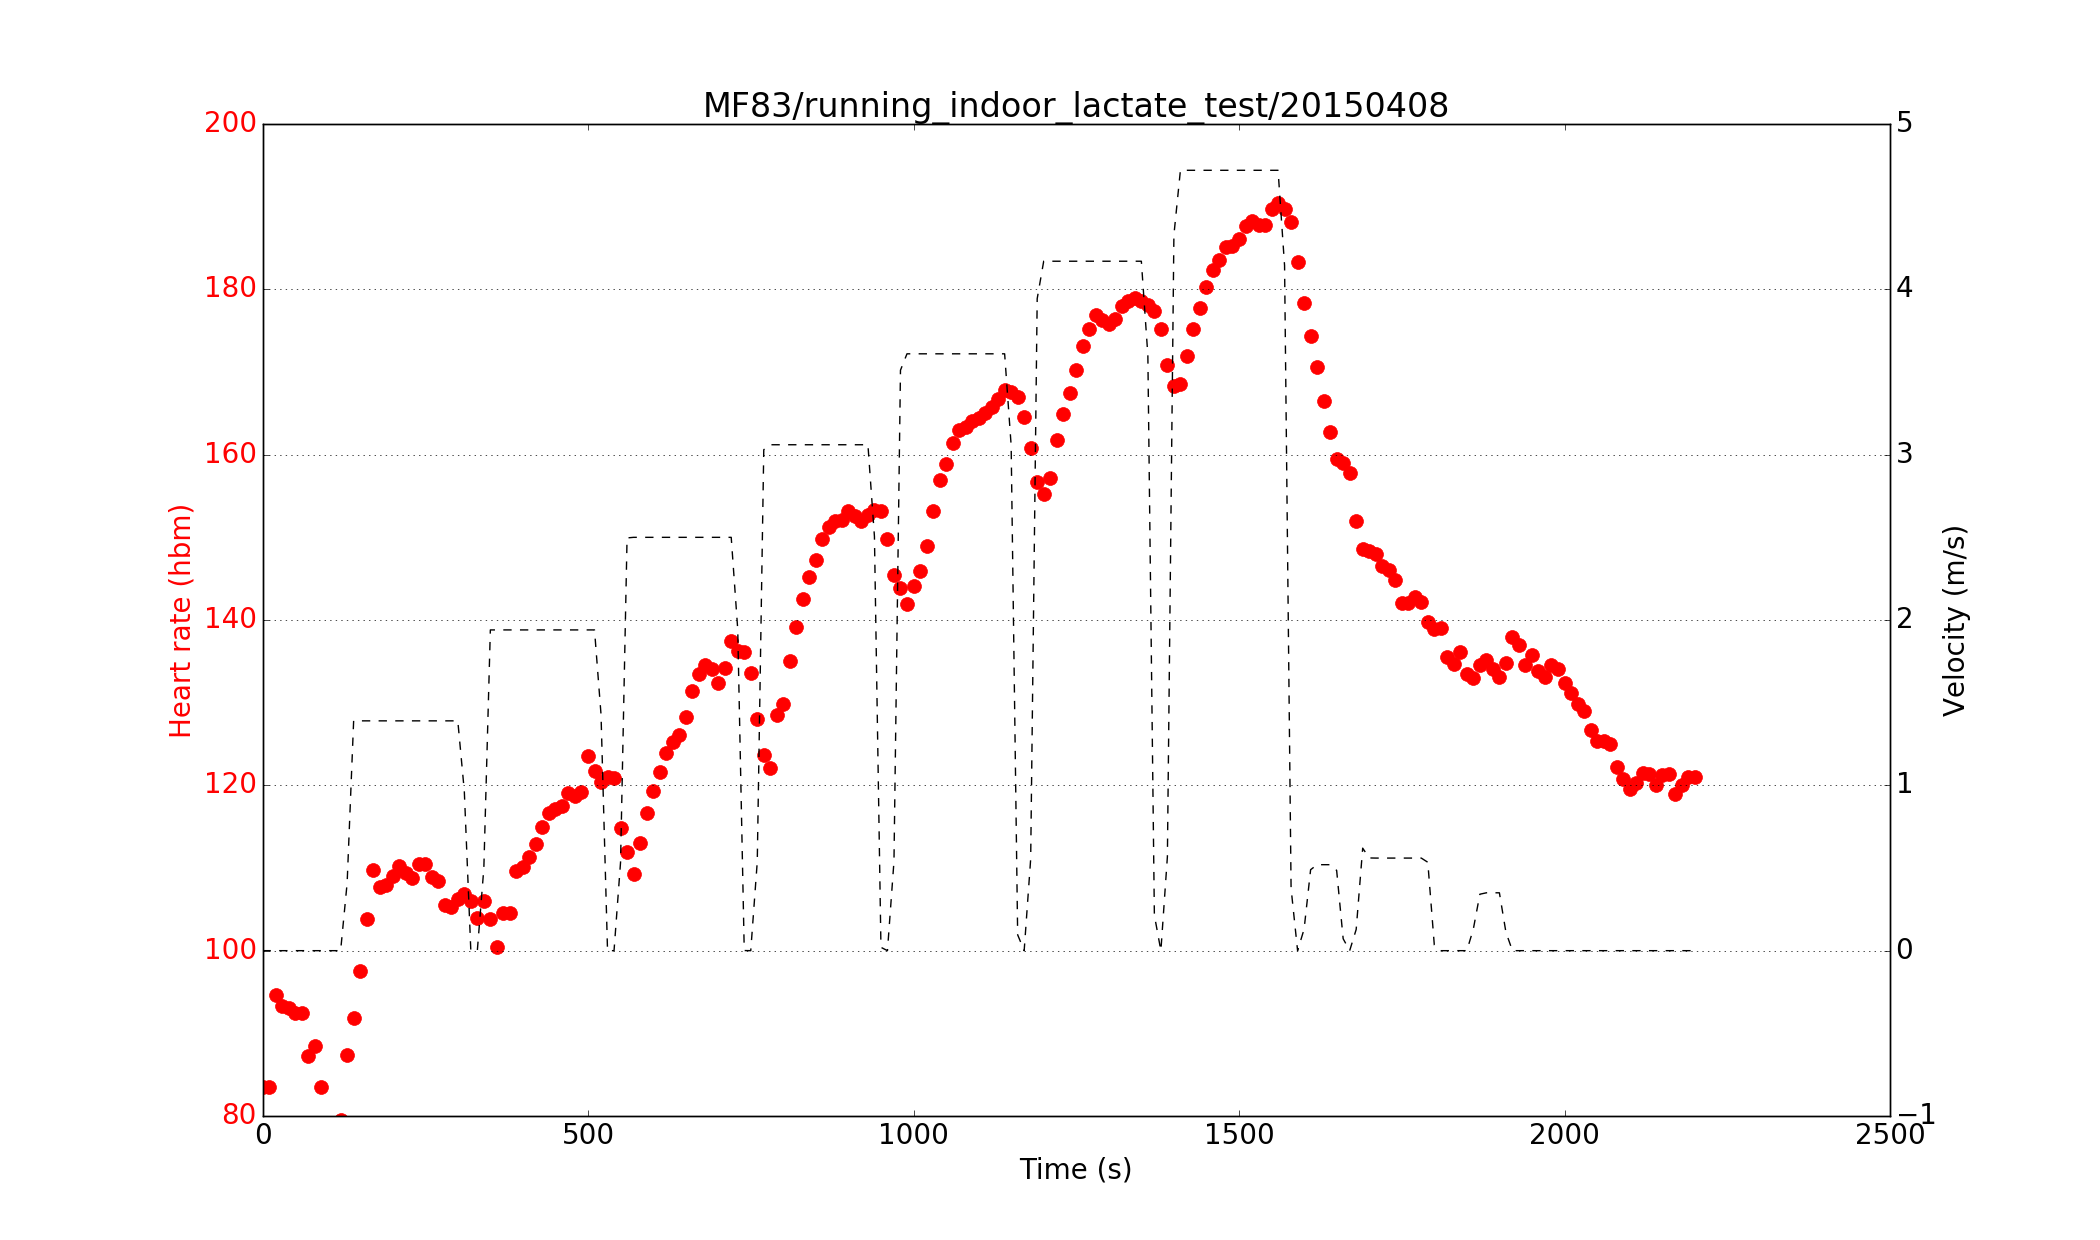
\includegraphics[height=6cm]{../images/plot_hbm_velocity-lactate.png}
    \end{subfigure}
    \\
    \begin{subfigure}{\textwidth}
        \centering
        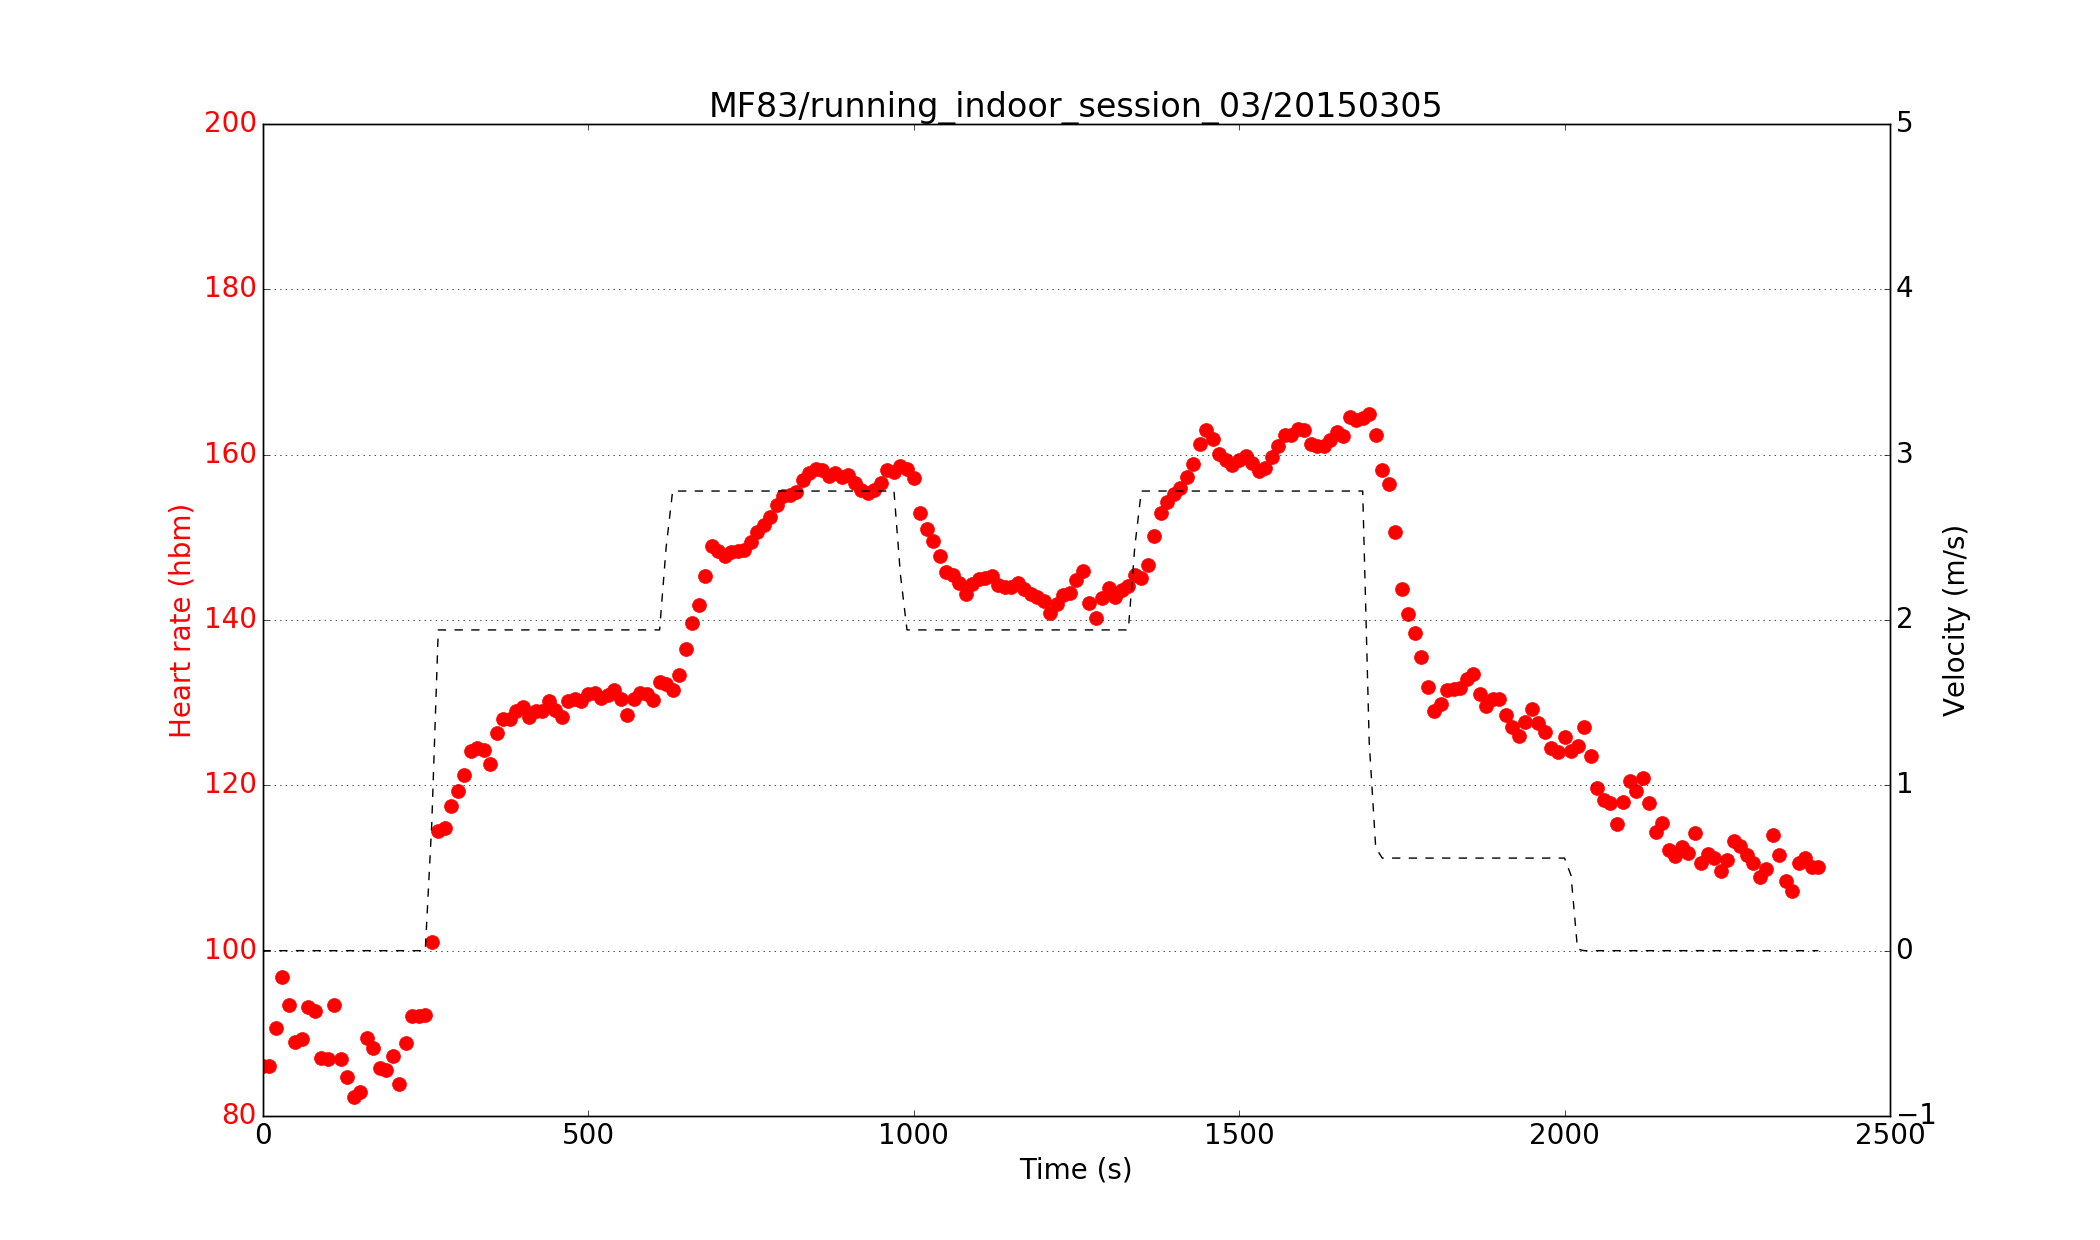
\includegraphics[height=6cm]{../images/plot_hbm_velocity-session3.png}
    \end{subfigure}
    \caption{Heart rate and velocity recorded for a sample session of each exercise type: onset/offset, step protocol, and interval exercise} \label{fig:data}
\end{figure}
\subsection{Data set}
    The experiments were conducted on indoor running exercise data from F\"{u}ller et al..
    \begin{itemize}
        \item Three distinct types of exercises were recorded: an onset/offset exercise, a step exercise protocol, and an interval protocol. Details about how each exercise type are conducted can be found in the original paper \cite{Fueller15}. Figure \ref{fig:data} plots examples of the three types of exercises recorded. Three sessions are recorded for each type of exercise.
        \item The same preprocessing method is adopted from \cite{Fueller15}: data were down sampled to 10-second intervals from the original 1-second intervals.
    \end{itemize}

    \subsection{Experiment setup}
    \begin{figure}[H]
        \centering
        \begin{subfigure}{0.4\textwidth}
            \centering
            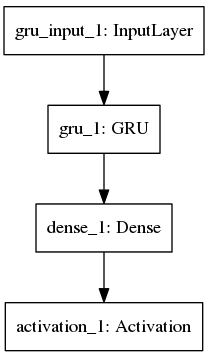
\includegraphics[width=0.9\linewidth]{../images/model_gru.png}
        \end{subfigure}%
        ~
        \begin{subfigure}{0.4\textwidth}
            \centering
            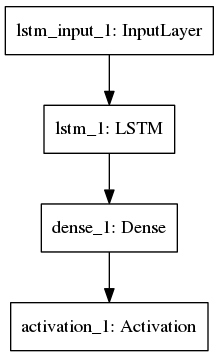
\includegraphics[width=0.9\linewidth]{../images/model_lstm.png}
        \end{subfigure}
        \caption{GRU and LSTM model as visualized by Keras} \label{fig:models}
    \end{figure}
    LSTM and GRU models from the Keras deep learning library are implemented for the prediction task.
    Biases of forget gates are initialized to ones as recommended by Jozefowicz et al. \cite{JozefowiczZS15}.

    The experiments are designed to observe the effects of the following parameters on the performance of the RNN LSTM model:
    \begin{itemize}
        \item Size of RNN lookback
        \item Number of neurons
        \item Optimization methods
    \end{itemize}

    \section{Results}

    \begin{figure}[H]
        \centering
        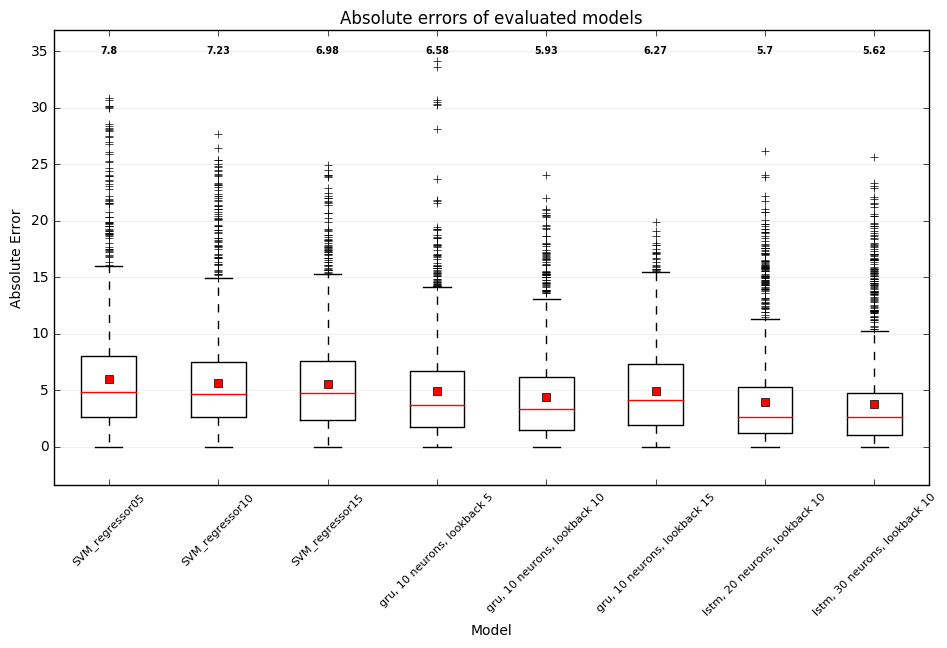
\includegraphics[width=\linewidth]{../images/plot_box_error_models.png}
        \caption{Box plot of absolute errors for each of the tested models. The numbers on top of each box is the cross-validated RMSE for the corresponding model.} \label{fig:box_error}
    \end{figure}
